% ══════════════════════════════════════════════════════════════════════════════
%  CHAPTER 6: BIG BANG NUCLEOSYNTHESIS
% ══════════════════════════════════════════════════════════════════════════════

\chapter{Big Bang Nucleosynthesis(BBN) (Lecture 13-14)}
\quad After electron-positron annihilation, light nuclei can form and survive without being immediately photodissociated by the high-energy photons in the early universe. \\

This process, known as Big Bang Nucleosynthesis (BBN), occurred within the first few minutes after the Big Bang($ T \sim 0.1 \text{ MeV} $) and is responsible for the formation of light elements such as deuterium, helium-3, helium-4, and lithium-7. \\

The abundances of these elements provide crucial evidence for the Big Bang model and allow us to test our understanding of the early universe's conditions and evolution.

% =══════════════════════════════════════════════════════════════════════════════
\bigskip
\section{Equilibrium}
% ──────────────────────────────────────────────────────────────────────────────
\subsection{binding energy}
\begin{intuition}
    Due to exist of strong interaction fore, the nucleus is more stable than its constituent nucleons in free state, so if we want to disassemble a nucleus into free protons and neutrons, we need to provide energy to overcome the binding energy of the nucleus, and we call it \textbf{binding energy}. \\

    On the other hand, when we said a nucleus is more stable than its constituent nucleons, thats means it is in a lower energy state than the free nucleons, so we will expect the mass of the nucleus $m_i$ is less than the sum of the masses of its constituent protons and neutrons, which is $Z_i m_{^{1}H} + N_i m_n$. \\
\end{intuition}

\bigskip \noindent
\begin{foundation}
    For a nuclei of species $i$ with $A_i$ Atomic Mass Number, it has below relationship:
    \[
        A_i = Z_i + N_i
    \],
    which $Z_i$ and $N_i$ are the number of protons and neutrons in the nucleus respectively. \\
\end{foundation}


\bigskip \noindent
\begin{theory}
    The binding energy of the nucleus of species $i$ is given by:
    \[
        B_i = Z_i m_{^{1}H} + N_i m_n - m_i
    \]
    where $Z_i$ and $N_i$ are the number of protons and neutrons in the nucleus, $m_{^{1}H}$ is the mass of a hydrogen atom, $m_n$ is the mass of a neutron, and $m_i$ is the mass of the nucleus of species $i$. \\
    
    We sometime also use the approximation of $m_{^{1}H} \approx m_p$ where $m_p$ is the mass of a proton, since the difference between the two is negligible for our calculations.
\end{theory}

% ──────────────────────────────────────────────────────────────────────────────
\bigskip \noindent \bigskip \noindent \bigskip \noindent
\subsection{number density of nuclei in chemical equilibrium}
\begin{foundation}
    Notes the proton, neutron, and electron in this stage are all non-relativistic, so we can use the Maxwell-Boltzmann distribution to describe their number densities. Recall:
    \[
        n_i = g_i \left( \frac{m_i k_B T}{2\pi \hbar^2} \right)^{3/2} e^{-(m_i c^2 - \mu_i)/k_B T}
    \]
    with $g_p = g_n = 2$, we can further rearrange the expression to get:
    \begin{align*}
        n_i &= g_i \left( \frac{m_i T}{2 \pi} \right)^{3/2} e^{(\mu_i - m_i) / T} \\
        e^{\mu_i/ T} &= \frac{n_i}{g_i} \left( \frac{2\pi}{m_i T} \right)^{3/2} e^{m_i / T}
    \end{align*}

    At the sametime, if the nuclear reactions are occur fast enough, we can assume the system is in chemical equilibrium:
    \[
        (A_i - Z_i) n + Z_i p \leftrightarrow i
    \]
    And hence the chemical potentials satisfy:
    \[
        (A_i - Z_i) \mu_n + Z_i \mu_p = \mu_i
    \] \\

    \pagebreak
    Sub the chemical potential relation into the number density expression, we can get:
    \begin{align*}
        n_i &= g_i \left( \frac{m_i T}{2 \pi}^{3/2} \right)e^{\frac{Z_i \mu_p + (A_i - Z_i) \mu_n - m_i}{T}}  \\
            &= g_i \left( \frac{m_i T}{2 \pi} \right)^{3/2} e^{\frac{Z_i \mu_p}{T}} e^{\frac{(A_i - Z_i) \mu_n}{T}} e^{-\frac{m_i}{T}} \\ 
            &= g_i \left( \frac{m_i T}{2 \pi} \right)^{3/2} \left( \frac{n_p}{g_p} (\frac{2\pi}{m_p T})^{3/2} e^{m_p / T} \right)^{Z_i} \left( \frac{n_n}{g_n} (\frac{2\pi}{m_n T})^{3/2} e^{m_n / T} \right)^{A_i - Z_i} e^{-m_i / T} \\
            &= g_i \left( \frac{m_i T}{2 \pi} \right)^{3/2} \frac{n_p}{g_p}^{Z_i} \frac{n_n}{g_n}^{A_i - Z_i} \frac{2\pi}{m_p T}^{3Z_i / 2} \frac{2\pi}{m_n T}^{3(A_i - Z_i) / 2} e^{(Z_i m_p + (A_i - Z_i) m_n - m_i) / T} \\
            &= g_i \left( \frac{m_i T}{2 \pi} (\frac{2\pi}{m_p T})^{Z_i} (\frac{2\pi}{m_n T})^{A_i - Z_i} \right)^{3/2} \left(n_p^{Z_i} n_n^{A_i - Z_i}\right) \left( g_p^{-Z_i} g_n^{-(A_i - Z_i)} \right) \left( e^{B_i / T} \right) \\
            &= g_i \left( (\frac{2\pi}{T})^{A_i - 1} \frac{m_i}{m_p^{Z_i} m_n^{A_i - Z_i}} \right)^{3/2} \left(n_p^{Z_i} n_n^{A_i - Z_i}\right) \left( 2^{-Z_i} 2^{-(A_i - Z_i)} \right) \left( e^{B_i / T} \right) \\
            &= g_i \left( (\frac{2\pi}{T})^{A_i - 1} \frac{m_N}{m_N^{Z_i} m_N^{A_i - Z_i}} \right)^{3/2} \left(n_p^{Z_i} n_n^{A_i - Z_i}\right) \left( 2^{-A_i} \right) \left( e^{B_i / T} \right) \\
            &= g_i \left( \frac{2\pi}{T}^{A_i - 1} \frac{A_i}{m_N} \right)^{3/2} \left(n_p^{Z_i} n_n^{A_i - Z_i}\right) 2^{-A_i} e^{B_i / T} \\
            &= g_i A_i^{3/2} \left( \frac{2\pi}{m_N T} \right)^{\frac{3}{2}(A_i - 1)} \left(n_p^{Z_i} n_n^{A_i - Z_i}\right) 2^{-A_i} e^{B_i / T}
    \end{align*}
    where we have used the approximation of $m_p \approx m_n \approx \frac{m_i}{A_i} \equiv m_N$ in the last step. \\
\end{foundation}

\bigskip \noindent
\begin{theory}
    The number density of species $i$ can be expressed as:
    \[
        n_i = g_i \cdot \left(A_i^{3/2} 2^{-A_i}\right) \cdot  \left(n_p^{Z_i} n_n^{A_i - Z_i}\right) \cdot \left( (\frac{2\pi}{m_N T})^{\frac{3}{2}(A_i - 1)} e^{B_i / T} \right)
    \]
    where $m_N$ is the average nucleon mass.
\end{theory}


% ──────────────────────────────────────────────────────────────────────────────
\clearpage
%\bigskip \noindent \bigskip \noindent \bigskip \noindent
\subsection{abundance of nuclei in chemical equilibrium}
\begin{theory}
    The abundance of species $i$ is defined as the ratio of its number density to the total baryon number density:
    \[
        X_i = \frac{A_i n_i}{n_B}
    \]
    where $n_B$ is the total baryon number density, which can be expressed as:
    \[
        n_B = \sum_i A_i n_i = n^{*}_p + n^{*}_n
    \]
    where $n^{*}_p$ and $n^{*}_n$ are the total number densities of protons and neutrons, respectively, including \textbf{both free and nuclei states}. To distinguish between the two, we often use the notation $n_p$ and $n_n$ for the free nucleon densities. \\
\end{theory}

\bigskip \noindent
\begin{foundation}
    Start from equations of number density of a nucleus i:
    \[
        n_i = g_i \cdot \left(A_i^{3/2} 2^{-A_i}\right) \cdot  \left(n_p^{Z_i} n_n^{A_i - Z_i}\right) \cdot \left( (\frac{2\pi}{m_N T})^{\frac{3}{2}(A_i - 1)} e^{B_i / T} \right)
    \] \\

    Let $n_p$ and $n_n$ be the number density of free protons and neutrons, we can get:
    \begin{align*}
        \begin{cases}
            X_i = \frac{A_i n_i}{n_B} \\
            X_p = \frac{n_p}{n_B} \\
            X_n = \frac{n_n}{n_B}
        \end{cases}
    \end{align*}
    with $n_B = n_p + n_n + \sum_i A_i n_i$.\\

    Substituting the expression of $n_i$ into the number density of species $i$, we can get:
    \begin{align*}
        \frac{X_i n_B}{A_i} &= g_i \cdot \left(A_i^{3/2} 2^{-A_i}\right) \cdot  \left((X_p n_B)^{Z_i} (X_n n_B)^{A_i - Z_i}\right) \cdot \left( (\frac{2\pi}{m_N T})^{\frac{3}{2}(A_i - 1)} e^{B_i / T} \right) \\
        \frac{X_i}{A_i} &= g_i \cdot \left(A_i^{3/2} 2^{-A_i}\right) \cdot  \left(X_p^{Z_i} X_n^{A_i - Z_i}\right) \cdot \left( (\frac{2\pi}{m_N T})^{\frac{3}{2}(A_i - 1)} e^{B_i / T} \right) n_B^{A_i - 1} \\
        X_i &= g_i \cdot \left(A_i^{5/2} 2^{-A_i}\right) \cdot  \left(X_p^{Z_i} X_n^{A_i - Z_i}\right) n_B^{A_i - 1} \cdot \left( (\frac{2\pi}{m_N T})^{\frac{3}{2}(A_i - 1)} e^{B_i / T} \right) 
    \end{align*} \\

    Now introduce the dimensionless parameter $\epsilon$ that characterizes the nucleon density phase space:
    \begin{align*}
        \epsilon &= \frac{1}{2} n_B \left( \frac{2\pi}{m_N T} \right)^{3/2} \\
    \end{align*}
    By using definition of Baryon-photon ratio $n_B = n_\gamma \eta$, and given the blackbody photon number density $n_\gamma = \frac{2\zeta(3)}{\pi^2} T^3$, we can further express $\epsilon$ as:
    \begin{align*}
        \epsilon &= \frac{1}{2} n_B \left( \frac{2\pi}{m_N T} \right)^{3/2} \\
        &= \frac{1}{2} n_\gamma \eta \left( \frac{2\pi}{m_N T} \right)^{3/2} \\
        &= \frac{1}{2} \cdot \frac{2\zeta(3)}{\pi^2} T^3 \cdot \eta \cdot \left( \frac{2\pi}{m_N T} \right)^{3/2} \\
        &= \frac{\zeta(3) \eta}{\pi^2} \left( \frac{2\pi T}{m_N} \right)^{3/2} 
    \end{align*} \\

    Hence, we can further rearrange the expression to get:
    \begin{align*}
        X_i &= g_i \cdot \left(A_i^{5/2} 2^{-A_i}\right) \cdot  \left(X_p^{Z_i} X_n^{A_i - Z_i}\right) \cdot \left( 2^{A_i - 1} n_B^{A_i - 1} (\frac{2\pi}{m_N T})^{\frac{3}{2}(A_i - 1)} e^{B_i / T} \right) \\
            &= g_i \cdot \left(A_i^{5/2} 2^{-A_i+ A_i - 1}\right) \cdot  \left(X_p^{Z_i} X_n^{A_i - Z_i}\right) \cdot \left( \epsilon^{A_i - 1} e^{B_i / T} \right) \\
            &= \frac{1}{2} g_i \cdot \left(A_i^{5/2} \epsilon^{A_i - 1}\right) \cdot \left(X_p^{Z_i} X_n^{A_i - Z_i}\right) \cdot e^{B_i / T}
    \end{align*}
\end{foundation}

\bigskip \noindent
\begin{theory}
   the relic abundance of species $i$ can be expressed as:
    \[
        X_i = \frac{A_i n_i}{n_B} = \frac{1}{2}g_i \cdot \left(A_i^{5/2} \epsilon^{A_i - 1}\right) \cdot \left( X_p^{Z_i} X_n^{A_i - Z_i} \right) \cdot e^{B_i / T}
    \]
    with:
    \[
        \epsilon = \frac{1}{2} n_B \left( \frac{2\pi}{m_N T} \right)^{3/2} = \frac{\zeta(3) \eta}{\pi^2} \left( \frac{2\pi T}{m_N} \right)^{3/2} 
    \],
    where $\epsilon$ is the dimensionless measure of density in phase space, and $\eta$ is the baryon-to-photon ratio. \\

    And we can get the relationship of $\epsilon$ and $\eta$:
    \[
        \epsilon \sim \frac{T}{m_N}^{3/2} \eta
    \]
\end{theory}

%\bigskip \noindent
\begin{remark}
    The relic abundance $X_i$ depends on two important factors: the Baryon-to-photon ratio $\eta$ and the Neutron-to-proton ratio $X_n / X_p$. The former determines the overall density of baryons in the universe, while the latter determines the relative abundance of neutrons and protons, which in turn affects the formation of different nuclei during BBN. \\
\end{remark}

% ──────────────────────────────────────────────────────────────────────────────
\bigskip \noindent \bigskip \noindent \bigskip \noindent
\section{Baryon-to-photon ratio}
\begin{theory}
    The baryon-to-photon ratio $\eta$ is a crucial parameter in cosmology that quantifies the relative abundance of baryons (protons and neutrons) to photons in the universe. It is defined as:
    \[
        \eta = \frac{n_B}{n_\gamma}
    \]
    By the CMB measurements, we have $\eta \approx 6 \times 10^{-10}$, which is a extremely small number. 
\end{theory}
\begin{remark}
In fact, the non-zero value of $\eta$ is a key piece of evidence for the matter-antimatter asymmetry in the universe, which allow matter to exist and form structures like galaxies, stars, and planets.\\

If $\eta$ were zero, we would expect equal amounts of matter and antimatter to annihilate each other, leaving behind a universe filled with radiation and no matter. The observed value of $\eta$ indicates that there is a slight excess of baryons over antibaryons in the early universe, which has profound implications for our understanding of the fundamental physics governing the universe's evolution.
\end{remark}

\clearpage
%\bigskip \noindent 
\begin{figure}[h]
    \centering
    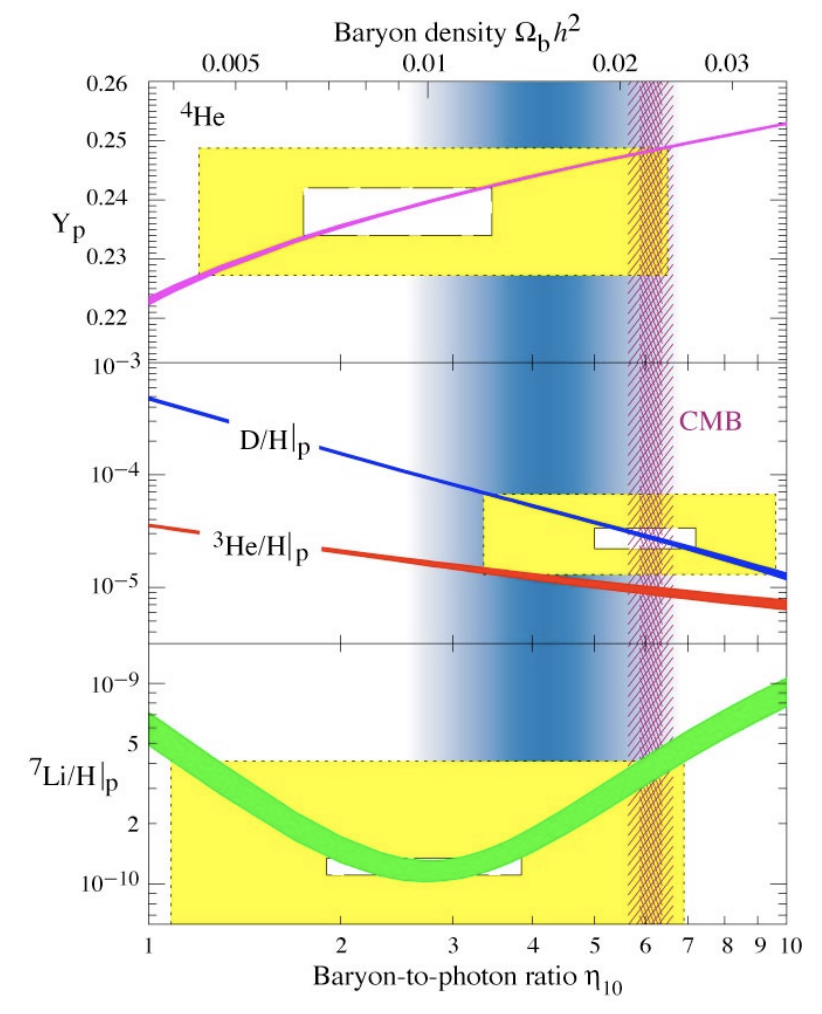
\includegraphics[width=0.5\textwidth]{images/baryon_to_photon_ratio.png}
    \caption{Baryon-to-photon ratio $\eta$, with x-axis is in unit of $10^{-10}$.}
    \label{fig:baryon_to_photon_ratio}
\end{figure}

\begin{extra}
    From the figure above, the x-axis is different initial condition of universe that with different baryon-to-photon ratio $\eta$, and the y-axis is the corresponding relic abundance that we can observe if the universe has that initial condition. The 4 different lines from up to down represent the abundance of helium-4, deuterium, helium-3, and lithium-7 predicted by the BBN theory respectively. \\

    The vertical band in the figure represents the observed value of $\eta$ from CMB($t \sim 380,000$ years) measurements, which is around $6 \times 10^{-10}$. While the yellow/white box represents the observed abundances($t \sim 3-20$ minutes) of the 3 light elements (helium-4, deuterium, and lithium-7) from astrophysical observations. The White box represents a precise measurement values, while the yellow box cover a higher confidence level. \\
    
    We can see that the for the upper two box the theoretical line cross the box at the CMB band, the upper and lower bound of measurement values(i.e. top and bottom edge of the white box) are similar to the value of the line at the CMB band($0.23-0.24$ v.s. $0.25$ for helium-4, and both around $5 \times 10^{-5}$ for deuterium); However, for the lithium-7, the value of the line at the CMB band $4\times 10^{-10}$ is much higher than the observed value, which is around $1 \times 10^{-10}$, and this discrepancy is known as the "lithium problem" in cosmology. \\
\end{extra}




% ──────────────────────────────────────────────────────────────────────────────
\bigskip \noindent \bigskip \noindent \bigskip \noindent
\section{Neutron-to-Proton Ratio}
\begin{theory}
    The neutron-proton interaction occurs through weak interaction:
    \begin{align*}
        n + e^+ &\leftrightarrow p + \bar{\nu}_e \\
        n + \nu_e &\leftrightarrow p + e^- \\
    \end{align*}

    Consider the chemical equilibrium of the above reactions, we can get:
    \[
        \mu_n + \mu_{\nu_e} &= \mu_p + \mu_{e^-} 
    \]
    and by dividing the two number density expressions of neutron and proton, we can get:
    \[
        \frac{n_n}{n_p} = e^{\frac{-(m_n - m_p)}{T} + \frac{\mu_{\nu_e} - \mu_{e^-}}{T}} 
    \]
\end{theory}

\bigskip \noindent
\begin{foundation}
    To estimate the chemical potential of neutrino and electron, we assume $T > m_e$, and have:
    \begin{align*}
        n_{e^-} - n_{e^+} &= \frac{2}{2\pi^2} \int_0^\infty \left(\frac{1}{e^{\frac{E_{e^-} - \mu_{e^-}}{T}} + 1} - \frac{1}{e^{\frac{E_{e^+} - \mu_{e^+}}{T}} + 1}\right) E^2 dE \\
        &= \frac{2 T^3}{6 \pi^2} \left( \pi^2 \frac{\mu_{e^-}}{T} + \left( \frac{\mu_{e^-}}{T} \right)^3 \right)
    \end{align*}
    and as the universe is electrically neutral, we have $n_{e^-} - n_{e^+} = n_p^*$, and by $n_B = n_p^* + n_n^*$, we can get:
    \begin{align*}
        n_{e^-} - n_{e^+} &< n_B \\
        n_{e^-} - n_{e^+} &< \eta n_\gamma  \\
        n_{e^-} - n_{e^+} &< \eta \cdot \frac{2\zeta(3)}{\pi^2} T^3
    \end{align*}

    Now sub the inequality back to the expression of $n_{e^-} - n_{e^+}$, we can get:
    \begin{align*}
        \frac{2 T^3}{6 \pi^2} \left( \pi^2 \frac{\mu_{e^-}}{T} + \left( \frac{\mu_{e^-}}{T} \right)^3 \right) &< \eta \cdot \frac{2\zeta(3)}{\pi^2} T^3 \\
        \frac{1}{6} \left( \pi^2 \frac{\mu_{e^-}}{T} + \left( \frac{\mu_{e^-}}{T} \right)^3 \right) &< \eta \cdot \zeta(3) \\
        \frac{\mu_{e^-}}{T} + \frac{1}{\pi^2}\left( \frac{\mu_{e^-}}{T} \right)^3 &< \frac{6 \eta}{\pi^2} \zeta(3)
    \end{align*}

    Note that $\eta$ is around $6 \times 10^{-10}$, we can get $\frac{\mu_{e^-}}{T} < 10^{-9}$, which is negligible; At the same time, we know that the neutrino asymmetry is small through observations of CMB and BBN, so through a similar calculation, we can also get $\frac{\mu_{\nu_e}}{T} < 10^{-9}$, which is also negligible.
\end{foundation}

\bigskip \noindent
\begin{theory}
    If further considering the energy scale of BBN $T \sim 0.1 \text{ MeV}$, we can just ignore the chemical potential of neutrino and electron, and hence we can get the neutron-to-proton ratio as:
    \[
        \frac{n_n}{n_p} = e^{\frac{-(m_n - m_p)}{T}} 
    \] 
    where $m_n - m_p \approx 1.293 \text{ MeV}$. \\

    The reaction continue until expansion of universe outcomes the reaction rate, which happens at around $T \sim 0.7 \text{ MeV}$, which called "freeze-out" temperature; and at freeze-out, the ratio is around $1/7$ at the start of BBN.
\end{theory}




% =══════════════════════════════════════════════════════════════════════════════
\bigskip \noindent \bigskip \noindent \bigskip \noindent
\section{BBN processes}
\subsection{Deuterium Bottleneck Effect and Start of BBN}

\begin{figure}[htbp]
    \centering
    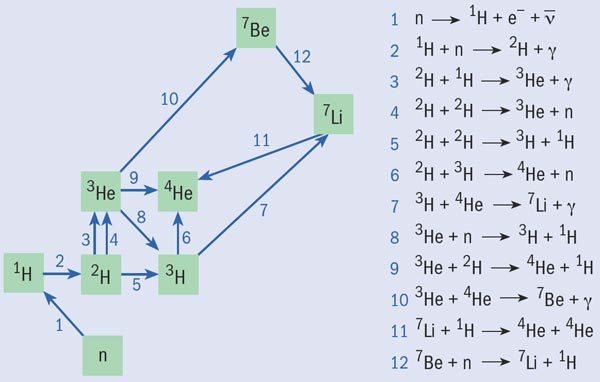
\includegraphics[width=0.8\textwidth]{images/BBN_interaction_chain.jpg}
    \caption{BBN interaction chain.}
    \label{fig:BBN_chain}
\end{figure}



% ──────────────────────────────────────────────────────────────────────────────
\bigskip \noindent \bigskip \noindent \bigskip \noindent
\subsection{Shutdown of BBN}

\begin{extra}
    \begin{center}
        \begin{tabular}{lrr}
        \toprule
        \textbf{} \qquad& \textbf{B(MeV)} \qquad & \textbf{B/A (MeV per u)} \\
        \midrule
        ${}^2\text{H}$ & 2.2245 & 1.11\\
        ${}^3\text{H}$ & 8.4820 & 2.83\\
        ${}^3\text{He}$ & 7.7186 & 2.57\\
        ${}^4\text{He}$ & 28.2970 & 7.07\\
        ${}^6\text{Li}$ & 31.9965 & 5.33\\
        ${}^7\text{Li}$ & 39.2460 & 5.61\\
        ${}^7\text{Be}$ & 37.6026 & 5.37\\
        ${}^{12}\text{C}$ & 92.1631 & 7.68\\
        ${}^{56}\text{Fe}$ & 492.2623 & 8.79\\
         \bottomrule
        \bottomrule
        \end{tabular}
    \end{center}
    \label{tab:binding_energies}
\end{extra}

% -─────────────────────────────────────────────────────────────────────────────
\bigskip \noindent \bigskip \noindent \bigskip \noindent
\subsection{Evolution of Elemental Abundances}

\begin{figure}[htbp]
    \centering
    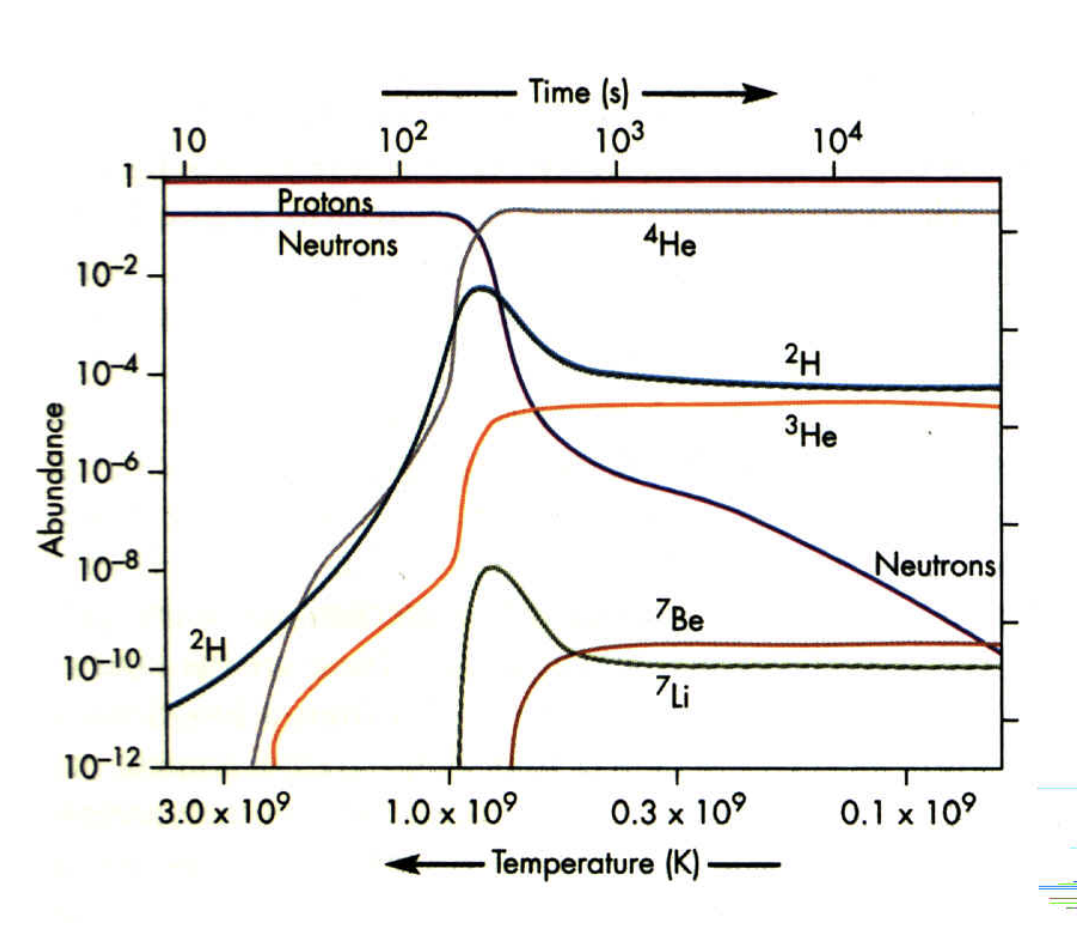
\includegraphics[width=0.8\textwidth]{images/time_evolution_abundance.png}
    \caption{Evolution of elemental abundances during BBN.}
    \label{fig:time_evolution_abundance}
\end{figure}

\begin{extra}
    The history of BBN research began with George Gamow's work in abundances of elements in the universe, he suggested that the early universe was hot and dense enough for nuclear reactions to occur, leading to the formation of light elements. His student Ralph Alpher further developed the theory through calculations. Later, in April 1, 1948, the results was announced in the letter to Physical Review , which signed by Alpher, Bethe, and Gamow, where Hans Bethe's name was added as a pun of "alpha, beta, gamma". 
\end{extra}